\documentclass[conference]{IEEEtran}
\IEEEoverridecommandlockouts
\usepackage{cite}
\usepackage{amsmath,amssymb,amsfonts}
\usepackage{mathtools}
\usepackage{algorithmic}
\usepackage{graphicx}
\usepackage{textcomp}
\usepackage{xcolor}
\usepackage{booktabs}
\usepackage{multirow}
\usepackage{url}

\def\BibTeX{{\rm B\kern-.05em{\sc i\kern-.025em b}\kern-.08em
    T\kern-.1667em\lower.7ex\hbox{E}\kern-.125emX}}

\begin{document}

\title{MonoArm: Anatomically Consistent Arm Joint Angle Estimation\\
from a Single RGB Camera for Real-Time Avatar Control}

\author{
\IEEEauthorblockN{Author Name Withheld for Draft}
\IEEEauthorblockA{\textit{Department (to be completed)} \\
\textit{Institution (to be completed)} \\
City, Country \\
email@domain.example}
}

\maketitle

\begin{abstract}
Soft wearable exoskeletons for upper-limb rehabilitation require joint
angle references for calibration and validation, but marker-based motion
capture is costly and lab-bound. We present MonoArm, a real-time
framework that estimates four anatomically consistent degrees of freedom
per arm -- shoulder flexion-extension, abduction-adduction,
internal-external rotation, and elbow flexion -- from a single RGB camera
and drives a rigged humanoid avatar in Unity. Joint angles are derived
from upper-arm and forearm direction vectors expressed in a Gram-Schmidt
orthonormalized torso frame and decomposed with a ZXY Euler sequence
chosen to relocate the parameterization's coordinate singularity away
from the arm-hanging rest pose, where the ISB-recommended YXY sequence is
degenerate. Shoulder axial rotation, which is unobservable from the
upper-arm vector alone, is estimated by a forearm-projection proxy that
is explicitly gated below $25^\circ$ of elbow flexion rather than
reported as a noise-dominated value. Three causal temporal filters
(moving average, Savitzky-Golay, and a two-state Kalman filter) are
implemented per channel and compared on a common jitter/lag benchmark; a
three-tier calibration maps raw estimates to a user's range of motion
under bounded-gain guards; and a UDP protocol streams filtered angles to
Unity's Humanoid muscle-space API. On a synthetic benchmark the Kalman
filter attains $0.55^\circ$ static standard deviation with no measurable
step lag, against $1.46^\circ$ and $133$~ms for a five-sample moving
average, and all configurations meet the $\pm3$--$5^\circ$ static-pose
target. A 55-case analytic test suite verifies the angle solver against
closed-form reference poses, torso-frame orthonormality, filter dynamics,
and cross-framework keypoint remapping; end-to-end inference with the
real MediaPipe landmarker on a real photograph produces bilateral angles
consistent with the observed pose. We report validation scope precisely:
all results here derive from analytic, synthetic, or single-image
verification, and quantitative accuracy against large-scale 3D
motion-capture ground truth (Human3.6M, CMU Panoptic Studio) was not
obtainable in our environment; the complete evaluation harness for that
comparison ships with the system and is documented for reuse.
\end{abstract}

\begin{IEEEkeywords}
monocular pose estimation, joint angle estimation, MediaPipe, Unity,
Kalman filter, rehabilitation robotics, wearable exoskeleton,
reproducibility
\end{IEEEkeywords}

\section{Introduction}

Restoring upper-limb function after stroke, spinal cord injury, or
neuromuscular disease typically demands repetitive, quantified therapy.
Soft wearable exoskeletons are increasingly proposed to deliver such
assistance safely and comfortably, but operating, evaluating, and
personalizing them requires a measurement of joint motion that is itself
trustworthy. Marker-based and multi-camera motion capture remain the
accuracy gold standard while being expensive, lab-bound, and impractical
for continuous or home use. Single-RGB-camera pose estimators --
MediaPipe Pose \cite{bazarevsky2020blazepose}, MoveNet
\cite{movenet2021blog}, and PersonLab-derived PoseNet
\cite{papandreou2018personlab} -- now track body keypoints from ordinary
webcam video, offering a low-cost, non-contact route to the same
reference signal.

Turning keypoints into a usable reference is not simply a matter of
running a detector. Raw landmark coordinates are camera-relative, so the
same physical shoulder pose yields different numbers under camera tilt or
subject lean; a naive Euler decomposition is singular precisely at the
pose a resting arm occupies most of the time; shoulder axial rotation is
geometrically unobservable from the upper-arm segment alone; and
keypoint-level jitter propagates into angle estimates that must
nonetheless drive an avatar smoothly. This paper addresses those four
problems concretely and reports what the resulting system does and does
not establish.

\subsection{Contributions}
\begin{enumerate}
\item A torso-relative, Gram-Schmidt orthonormalized coordinate frame and
a ZXY Euler decomposition that keeps the coordinate singularity away from
the arm-hanging rest pose, with a bilateral formulation that derives the
left arm by sagittal reflection rather than a duplicated sign convention
(Sections~\ref{sec:angles}--\ref{sec:bilateral}).
\item An explicitly gated forearm-projection estimator for shoulder axial
rotation, which reports a reliability flag rather than a noise-dominated
angle when the elbow is too extended for the estimate to be observable
(Section~\ref{sec:angles}).
\item A per-channel comparison of three causal filters on a common
static/step/sinusoid benchmark, treating filtering as an explicit
ablation factor so that smoothing effects are never conflated with
estimator accuracy (Section~\ref{sec:results-filters}).
\item A three-tier calibration with bounded-gain guards that prevent a
poorly-held reference pose from producing a runaway scale factor
(Section~\ref{sec:calibration}), plus a UDP-to-Unity muscle-space control
path that is avatar-agnostic (Section~\ref{sec:unity}).
\item A validation account that separates analytically verified claims,
synthetic benchmarks, and real-image verification from the dataset-scale
accuracy comparison we could not run, together with the harness that
would produce it (Sections~\ref{sec:results}--\ref{sec:limitations}).
\end{enumerate}

\section{Related Work}

\subsection{Monocular 2D Pose Estimation}
MediaPipe Pose builds on BlazePose \cite{bazarevsky2020blazepose}, a
two-stage detector-plus-regressor network predicting 33 pseudo-3D
landmarks under real-time CPU budgets. MoveNet \cite{movenet2021blog} is
a single-shot center-tracking architecture released in latency-optimized
(Lightning) and accuracy-optimized (Thunder) variants over COCO
17-keypoint output. The PoseNet variant used here is a TensorFlow Lite
MobileNetV1 heatmap-and-offset decoder whose bottom-up part grouping
derives from PersonLab \cite{papandreou2018personlab}. We integrate all
three behind one \texttt{PoseEstimator} interface, remapping COCO-17
outputs onto the MediaPipe 33-landmark indexing so that estimator
identity is a single swappable factor rather than a fork in the
downstream code.

\subsection{Anatomical Angle Extraction and Filtering}
Clinically meaningful joint angles require a body-relative frame. We
follow the intent of the ISB recommendation for shoulder and elbow
reporting \cite{wu2005isb}, substituting a ZXY Euler sequence for
numerical reasons detailed in Section~\ref{sec:angles}, and adopt the
two-link rigid-segment arm abstraction used in prior reconstructions of
arm kinematics from spatial tracking \cite{biryukova2000kinematics,
koritnik2003kinematic}. For smoothing we compare a two-state Kalman
filter \cite{kalman1960new} with Savitzky-Golay polynomial smoothing
\cite{savitzky1964smoothing} and a moving average.

\subsection{Benchmarks and Evaluation Practice}
Human3.6M \cite{ionescu2014human36m} is the standard 3D human pose
benchmark, providing 3.6M frames of synchronized video and MoCap-derived
joint positions across seven subjects, gated behind researcher
registration. CMU Panoptic Studio \cite{joo2015panoptic} is a 480-camera
dome system whose reconstructed 3D keypoints are partially distributed
without registration and are commonly used as a substitute. Mean
Per-Joint Angle Error (MPJAE) and Percentage of Correct Keypoints follow
the conventions of \cite{yang2011articulated, mehta2017vnect}. For
system comparison we use Wilcoxon signed-rank testing
\cite{wilcoxon1945individual}, Cohen's $d_z$ \cite{cohen1988statistical},
bootstrap confidence intervals, Holm-Bonferroni correction
\cite{holm1979simple}, and Bland-Altman agreement analysis
\cite{bland1986statistical}.

\section{Method}
\label{sec:method}

\subsection{Pipeline Overview}
A vision module captures monocular RGB frames and runs a selected pose
estimator. A processing module constructs a torso frame once per frame,
decomposes four joint angles per arm, applies one causal temporal filter
per channel (Section~\ref{sec:filtering}), and applies calibration. A Unity module receives the
resulting angle stream over UDP and drives a Humanoid-rigged avatar
through the muscle-space API, with an independent frame-rate-independent
smoothing stage.

\subsection{Torso Coordinate Frame}
From the four torso landmarks (left/right shoulder, left/right hip), with
$\mathbf{h}_{mid}$ and $\mathbf{s}_{mid}$ the hip and shoulder midpoints,
\begin{align}
\hat{\mathbf{y}} &= \operatorname{norm}(\mathbf{s}_{mid} - \mathbf{h}_{mid}) &&\text{(superior)}\\
\mathbf{x}_{c} &= \operatorname{norm}(\mathbf{s}_{L} - \mathbf{s}_{R}) &&\text{(lateral candidate)}.
\end{align}
Keypoint noise leaves $\mathbf{x}_c$ and $\hat{\mathbf{y}}$ only
approximately orthogonal, so one Gram-Schmidt step restores an exact
basis:
\begin{align}
\mathbf{x}' &= \mathbf{x}_c - (\mathbf{x}_c\cdot\hat{\mathbf{y}})\hat{\mathbf{y}}, &
\hat{\mathbf{z}} &= \operatorname{norm}(\mathbf{x}' \times \hat{\mathbf{y}}) \\
\hat{\mathbf{x}} &= \operatorname{norm}(\hat{\mathbf{y}} \times \hat{\mathbf{z}}). &&
\end{align}
This yields a right-handed frame
$R = [\hat{\mathbf{x}}\;\hat{\mathbf{y}}\;\hat{\mathbf{z}}]$ with
$\hat{\mathbf{x}}$ lateral (toward the subject's left),
$\hat{\mathbf{y}}$ superior, and $\hat{\mathbf{z}}$ anterior; world
vectors map to torso coordinates as
$\mathbf{v}_{torso} = R^{\!\top}\mathbf{v}_{world}$. Because all
downstream angles are expressed in this frame, camera tilt and torso lean
are compensated implicitly. Section~\ref{sec:results-analytic} verifies
$R^{\!\top}R = I$ and $\det(R) = +1$ numerically.

\subsection{Shoulder and Elbow Decomposition}
\label{sec:angles}
Let $\mathbf{v} = (v_x, v_y, v_z)$ be the unit upper-arm vector
(shoulder$\to$elbow) in torso coordinates. We decompose shoulder
orientation with a ZXY sequence rather than the ISB-recommended YXY
because YXY is singular exactly at $\mathbf{v}\approx(0,-1,0)$ -- the
arm-hanging rest pose, which dominates natural motion. ZXY moves that
pole to the arm pointing along the camera axis, a rarely-held pose, at
the cost of a second degeneracy at full abduction
(Section~\ref{sec:limitations}). Then
\begin{align}
\theta_{flex} &= \operatorname{atan2}(-v_z, -v_y) \\
\theta_{abd} &= \arcsin(\operatorname{clip}(-v_x, -1, 1)),
\end{align}
where the sign on $v_x$ reflects $\hat{\mathbf{x}}$ pointing toward the
subject's left. Elbow flexion follows from the upper-arm and forearm unit
vectors $\hat{\mathbf{u}}, \hat{\mathbf{f}}$ (both proximal$\to$distal):
\begin{equation}
\theta_{elbow} = \arccos(\operatorname{clip}(\hat{\mathbf{u}}\cdot\hat{\mathbf{f}}, -1, 1)),
\end{equation}
giving $0^\circ$ at full extension and increasing with flexion.

Axial rotation of the humerus does not move the elbow and is therefore
not recoverable from $\mathbf{v}$. We estimate it from the forearm's
component orthogonal to the upper-arm axis:
\begin{equation}
\mathbf{f}_\perp = \hat{\mathbf{f}} - (\hat{\mathbf{f}}\cdot\hat{\mathbf{u}})\hat{\mathbf{u}}, \quad
\theta_{rot} = \operatorname{atan2}(\mathbf{f}_\perp\!\cdot\!\mathbf{e}_1,\ \mathbf{f}_\perp\!\cdot\!\mathbf{e}_2)
\end{equation}
for an orthonormal basis $(\mathbf{e}_1, \mathbf{e}_2)$ of that plane.
The projection is well-conditioned only while $\|\mathbf{f}_\perp\|$ is
bounded away from zero, i.e.\ while the elbow is meaningfully bent. Below
$25^\circ$ of elbow flexion the system returns a placeholder with the
reliability flag cleared, so that consumers -- including the evaluation
harness -- can exclude geometrically meaningless samples instead of
averaging noise into a reported error.

\subsection{Bilateral Formulation}
\label{sec:bilateral}
Rather than duplicating the equations with flipped signs, the left arm's
torso-frame vectors are reflected across the sagittal plane,
$(v_x,v_y,v_z)\mapsto(-v_x,v_y,v_z)$, before the right-arm formulas are
applied unchanged. A reflected left arm is geometrically
indistinguishable from a right arm, so this yields mirrored anatomical
conventions (abduction positive away from the midline, internal rotation
positive) on both sides from one code path. Elbow flexion, being a dot
product, is reflection-invariant. The same reflection is applied in the
ground-truth extractors, so predictions and references always share one
angle space.

\subsection{Temporal Filtering}
\label{sec:filtering}
Three causal filters operate independently per channel. The moving
average $y[n]=\frac1W\sum_{k=0}^{W-1}x[n-k]$ is a baseline with
$(W\!-\!1)/2$ frames of group delay. Savitzky-Golay
\cite{savitzky1964smoothing} fits a degree-$p$ polynomial over a window
and evaluates it at the most recent sample, preserving curvature better
than a flat mean. The two-state Kalman filter models
$\mathbf{x}=[\theta,\dot\theta]^{\!\top}$ under constant velocity,
$F=\begin{bsmallmatrix}1&dt\\0&1\end{bsmallmatrix}$, $H=[1\ 0]$, with
discretized white-noise-acceleration process covariance
$Q = q\begin{bsmallmatrix}dt^4/4 & dt^3/2\\ dt^3/2 & dt^2\end{bsmallmatrix}$
and the standard recursion
\begin{align}
\mathbf{x}^- &= F\mathbf{x}, & P^- &= FPF^{\!\top}+Q \\
K &= P^-H^{\!\top}(HP^-H^{\!\top}+R)^{-1} \\
\mathbf{x} &= \mathbf{x}^- + K(z-H\mathbf{x}^-), & P &= (I-KH)P^-.
\end{align}
Carrying angular velocity in the state lets the predict step extrapolate
through fast motion, which is what reduces lag relative to a moving
average. Filter state resets at tracking-loss and sequence boundaries so
smoothing never spans a discontinuity.

\subsection{Calibration}
\label{sec:calibration}
Calibration proceeds in three tiers. Tier~1 records four static
reference poses (arm down; arm forward at $90^\circ$ flexion; arm to the
side at $90^\circ$ abduction; elbow bent to $90^\circ$) and fits a
per-DOF affine map
$\text{calibrated} = (\text{raw} + \text{offset})\times\text{gain}$,
where the offset zeroes the arm-down reading and the gain maps the
observed span onto the anatomical reference. Tier~2 refines the range
bounds from a free range-of-motion sweep. Tier~3 expands the stored range
online by $5^\circ$ whenever a live reading exceeds it, so the avatar
never hard-clips for a hypermobile user. State persists as JSON between
sessions.

Naive gain fitting is fragile: if the user holds the reference pose
poorly so that the observed span is small, $\text{gain} = 90^\circ /
\text{span}$ explodes -- a $5^\circ$ span yields an $18\times$ gain that
would scale every subsequent angle far out of range. We therefore refuse
to fit a gain below a $30^\circ$ minimum span, and clamp any fitted gain
to $[0.5, 2.0]$, falling back to unity and reporting the reason
otherwise. This matters beyond avatar aesthetics: the same affine
structure is what a wearable exoskeleton's joint encoders would need for
alignment to an anatomical zero, so an unbounded gain would propagate
directly into a device reference signal.

\subsection{Communication and Unity Integration}
\label{sec:unity}
The vision and rendering processes communicate over UDP at a configurable
rate (default $30$~Hz; specification minimum $20$--$30$~Hz), one
newline-terminated packet per pose. A single-arm packet carries
\texttt{S,<flex>,<abd>,<rot>,<elbow>}; a bilateral packet carries
\texttt{B,} followed by the right then left quadruple, with an untracked
side holding its last value rather than snapping to zero. On the Unity
side a background thread performs the blocking receive and publishes into
a lock-protected double buffer, so the render loop never blocks on
network I/O. Angles are mapped to Unity's normalized Humanoid muscle
space through a configurable per-DOF linear transform and a
\texttt{Mathf.SmoothDamp} stage; using \texttt{HumanPoseHandler} rather
than named bone transforms keeps the controller avatar-agnostic across
any Humanoid-rigged model.

\section{Evaluation Methodology}
\label{sec:eval-harness}

\subsection{Metrics}
For prediction/reference pairs $\{(p_i, g_i)\}_{i=1}^{N}$ -- frames
missing either signal are excluded, never imputed -- the harness computes
MAE, RMSE, signed bias, Pearson $r$, $R^2$, PCK at
$5^\circ/10^\circ/15^\circ$, and jitter (mean frame-to-frame
$|\Delta p|$). MPJAE is the macro-average of per-DOF MAE. All angular
differences use the circular form
$\Delta_{circ} = ((p-g)+180)\bmod 360 - 180$, so a trajectory crossing
the $\pm180^\circ$ branch cut of the \texttt{atan2}-based decomposition
is not charged an artificial $360^\circ$ error.

\subsection{Statistical Protocol}
Two systems evaluated on identical frames are compared with a paired
$t$-test and, given the heavy-tailed nature of pose error, the
distribution-free Wilcoxon signed-rank test over per-frame absolute
errors, with Cohen's $d_z$ as effect size, percentile bootstrap
confidence intervals, and Holm-Bonferroni correction across the resulting
family.

\subsection{Protocol and Validity Labeling}
Dataset-backed evaluation follows the Human3.6M standard split (tune on
S1/S5/S6/S7, select on S8, test once on S9/S11), with Leave-One-Subject-Out
available as an alternative and an explicit leakage assertion that raises
if a tuning subject reappears in the test set. The harness distinguishes
three prediction sources: \texttt{live} (real estimators on real frames,
the only publication-grade mode), \texttt{csv} (previously computed real
predictions), and \texttt{synthetic} (ground truth plus
literature-calibrated Gaussian noise, for pipeline verification only).
Synthetic runs are tagged \texttt{publication\_grade=false} in exported
metadata and emit a warning banner, so a simulated number cannot be
mistaken for a measured one. We apply the same labeling to every result
below.

\section{Results}
\label{sec:results}

\subsection{Analytic Correctness}
\label{sec:results-analytic}
The 55-case suite (\texttt{tests/test\_pose\_estimators.py},
\texttt{tests/test\_evaluation.py}) requires no camera, GPU, or external
dataset: it constructs landmark configurations with closed-form expected
angles and checks the solver against them. All 55 pass. The checks that
carry the claims of Section~\ref{sec:method} are:

\begin{itemize}
\item \textbf{Reference poses.} An arm hanging straight down yields
flexion, abduction, and elbow flexion each within $1^\circ$ of zero; an
arm horizontal in front yields $90^\circ$ flexion within $2^\circ$; an
arm horizontal at the side yields $90^\circ$ abduction within $2^\circ$;
a right-angled elbow yields $90^\circ$ flexion within $2^\circ$.
\item \textbf{Frame validity.} $R^{\!\top}R = I$ and $\det(R) = +1$ to
floating-point precision over randomized non-degenerate configurations;
degenerate input (collapsed shoulder or hip baseline) returns no frame
rather than a malformed one.
\item \textbf{Physical constraints and gating.} Elbow flexion is never
negative; shoulder rotation is flagged unreliable whenever elbow flexion
falls below the $25^\circ$ threshold.
\item \textbf{Filters.} The moving average reduces injected Gaussian
noise; the Kalman filter initializes to the first observation and
converges on a constant input; all filters clear state on \texttt{reset()}.
\item \textbf{Calibration guards.} A $5^\circ$ reference span yields
unity gain rather than the naive $18\times$; spans that would fit a gain
outside $[0.5, 2.0]$ are clamped; a zero span cannot divide by zero.
\item \textbf{Keypoint remapping.} MoveNet's COCO $(y, x, \text{score})$
ordering is correctly transposed into MediaPipe's $(x, y, z)$ convention
and each remapped joint lands at its documented index -- a silent
failure mode when two keypoint schemas are mixed.
\item \textbf{Metrics.} MAE tracks injected noise at the theoretical
$\sigma\sqrt{2/\pi}$; MPJAE equals the mean of per-DOF MAEs; PCK@$5^\circ$
decreases monotonically with noise.
\end{itemize}

\subsection{Temporal Filter Benchmark}
\label{sec:results-filters}
\texttt{scripts/compare\_filters.py} synthesizes a 400-sample, $30$~Hz
signal in three segments: a static hold at $45^\circ$ (samples 0--150,
for static variance), a step to $90^\circ$ (150--250, for response lag),
and a $1$~Hz sinusoidal sweep (250--400, for tracking fidelity).
Table~\ref{tab:filters} reports the resulting metrics and
Fig.~\ref{fig:filters} the generated traces.

\begin{table}[t]
\centering
\caption{Filter comparison on the synthetic $30$~Hz static/step/sinusoid
benchmark. Static Std is measured over the static-hold segment against
the project's $\leq 3$--$5^\circ$ target. RMSE is computed over the full
signal including the sinusoidal segment. $\downarrow$ lower is better.}
\label{tab:filters}
\begin{tabular}{@{}lcccc@{}}
\toprule
Filter & Static Std $\downarrow$ & Noise Red. & Step Lag $\downarrow$ & RMSE \\
       & (\textdegree) & (\%) & (ms) & (\textdegree) \\
\midrule
Moving Avg.\ ($W{=}5$)   & 1.46 & 57.2 & 133.3 & 6.07 \\
Moving Avg.\ ($W{=}9$)   & 1.01 & 70.5 & 266.7 & 10.35 \\
Savitzky-Golay (11,3)    & 2.89 & 15.3 & 33.3  & 3.43 \\
Kalman (responsive)      & \textbf{0.55} & 83.8 & \textbf{0.0} & 17.70 \\
Kalman (balanced)        & \textbf{0.55} & 84.0 & \textbf{0.0} & 19.88 \\
Kalman (smooth)          & \textbf{0.55} & \textbf{84.0} & \textbf{0.0} & 20.81 \\
\bottomrule
\end{tabular}
\end{table}

\begin{figure}[t]
\centering
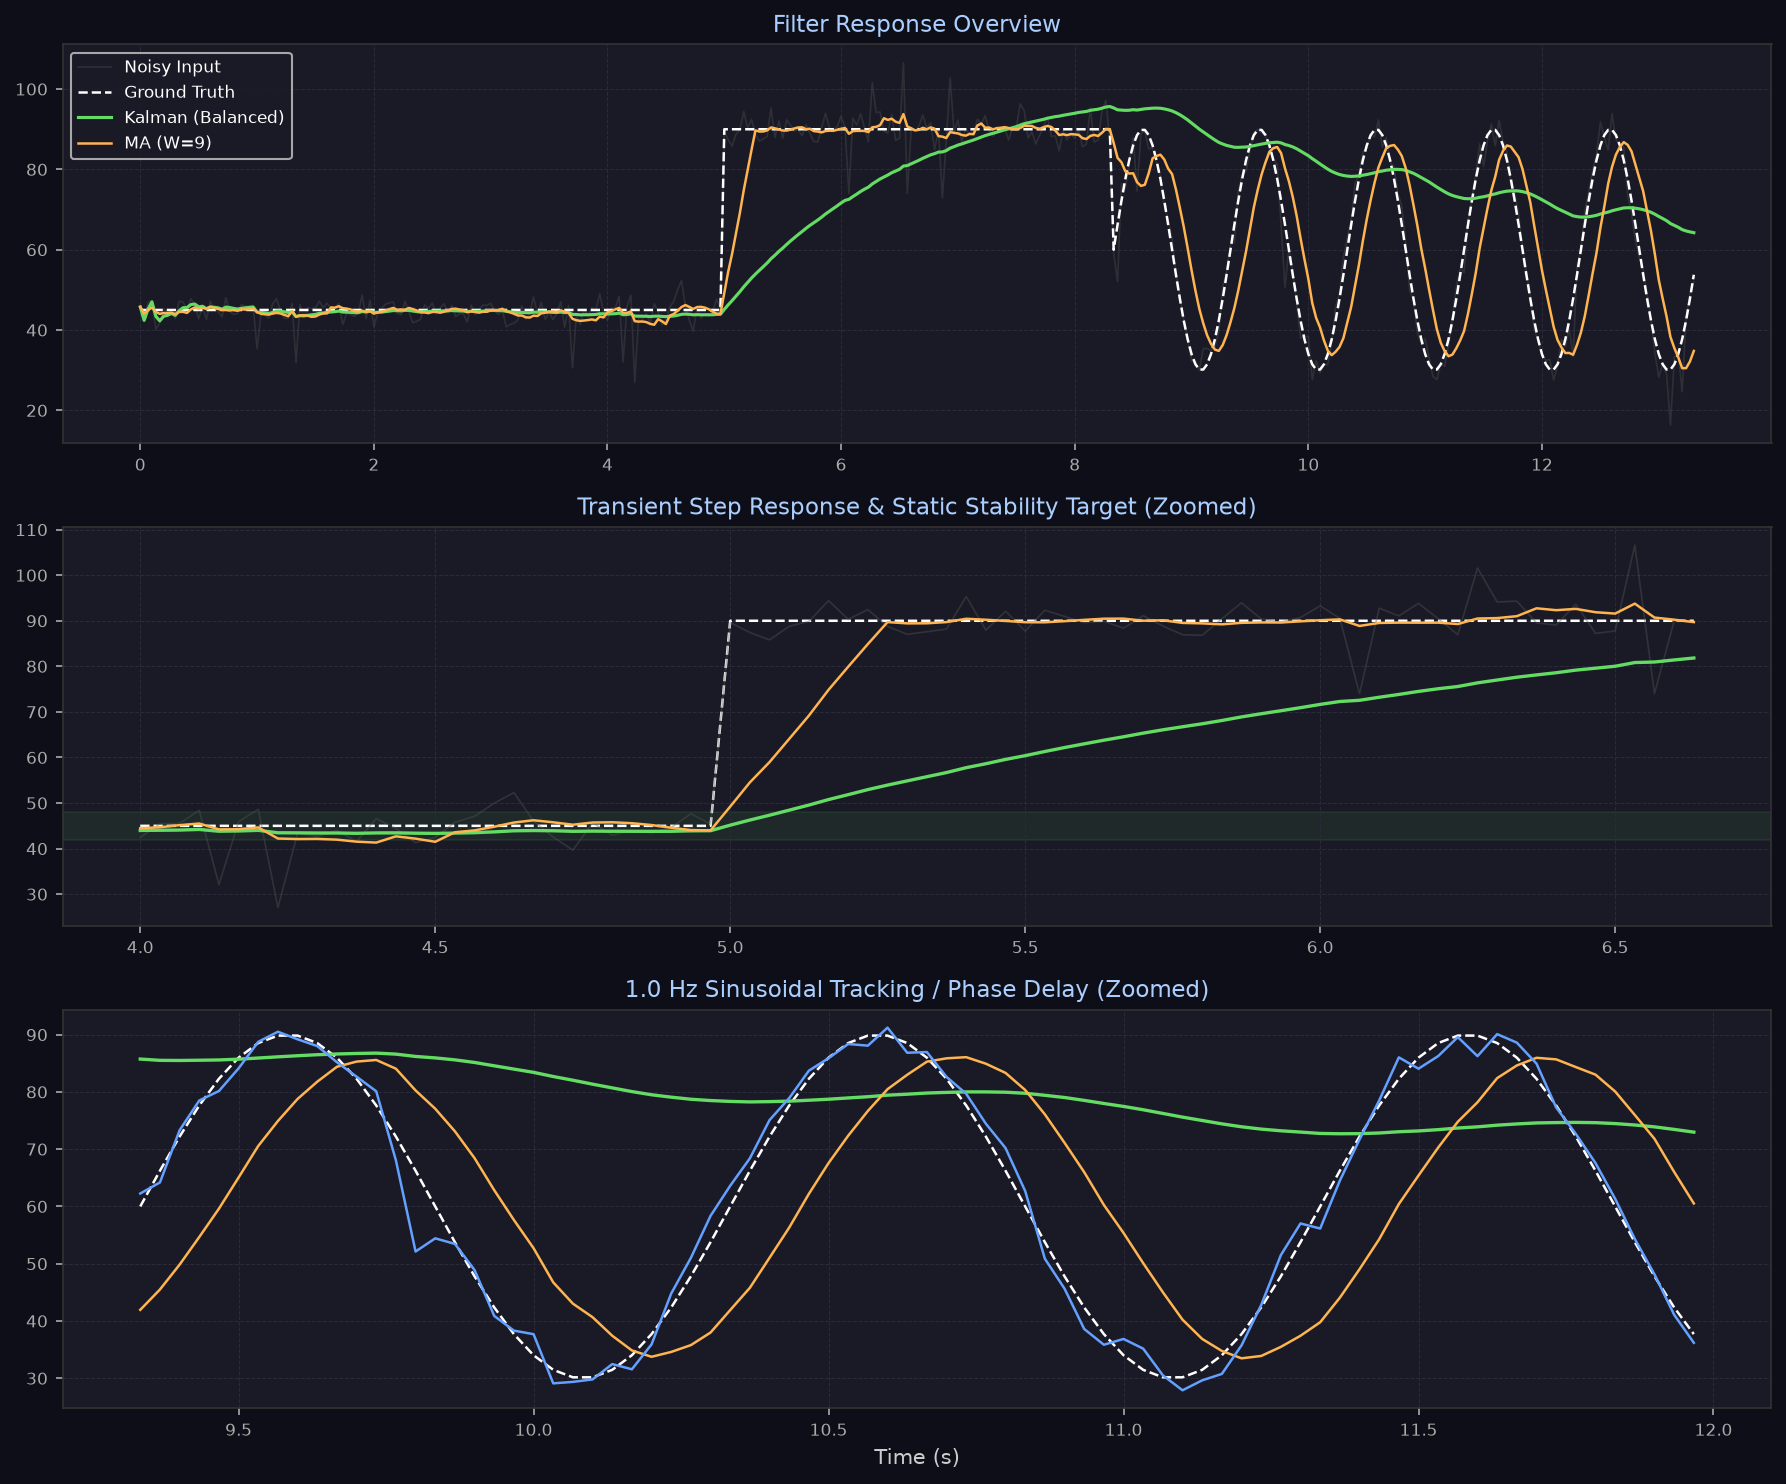
\includegraphics[width=\linewidth]{figures/filter_comparison.png}
\caption{Filter responses on the synthetic static/step/sinusoid benchmark
of Section~\ref{sec:results-filters}.}
\label{fig:filters}
\end{figure}

Every configuration satisfies the $\pm3$--$5^\circ$ static-pose target.
The Kalman filter reaches it with roughly a third of the five-sample
moving average's static deviation and no measurable step lag, because its
velocity state extrapolates through the transition instead of averaging
across it. Its full-signal RMSE is nonetheless the highest of the six.
This is not a contradiction but a property of the metric: RMSE here spans
the sinusoidal segment, where a responsive filter accumulates error from
faithfully following genuine motion while a heavily lagged filter can
score lower simply by under-reacting to a bounded oscillation.
Savitzky-Golay sits between the two extremes on both axes. Filter choice
is therefore a lag/smoothness trade-off rather than a scalar to minimize,
and the correct operating point depends on whether the consumer values
visual smoothness (avatar rendering) or fast-changing fidelity (a
controller reference).

\subsection{Occlusion Robustness}
\label{sec:results-occlusion}
\texttt{occlusion\_test.py --synthetic} generates 3{,}000 frames of
synthetic ground truth (independent per-DOF sinusoids), simulates each
estimator's raw output as ground truth plus a literature-calibrated
per-DOF Gaussian noise profile, occludes a fraction of frames at random,
and applies zero-order hold -- the behavior the live pipeline exhibits
when the estimator returns no detection. Table~\ref{tab:occlusion} and
Fig.~\ref{fig:occlusion} report the outcome. These noise profiles are
literature-calibrated approximations, not measurements of the three
frameworks, so this experiment characterizes pipeline mechanics under
data loss, not relative estimator accuracy.

\begin{table}[t]
\centering
\caption{Synthetic occlusion robustness ($n=3{,}000$ frames,
literature-calibrated noise profiles). Drift is the mean absolute
deviation of the held estimate from the true value during occluded frames
and is undefined at 0\% occlusion.}
\label{tab:occlusion}
\begin{tabular}{@{}llcccc@{}}
\toprule
Simulated profile & Occ.\ & Hold & MAE & RMSE & Drift \\
 & (\%) & (\%) & (\textdegree) & (\textdegree) & (\textdegree) \\
\midrule
MediaPipe & 0  & 0.0  & 2.59 & 3.26 & --   \\
MediaPipe & 25 & 25.0 & 2.60 & 3.27 & 0.83 \\
MediaPipe & 50 & 50.8 & 2.60 & 3.29 & 1.92 \\
MediaPipe & 75 & 75.3 & 2.56 & 3.23 & 2.76 \\
\midrule
MoveNet-Lightning & 0  & 0.0  & 4.30 & 5.40 & --   \\
MoveNet-Lightning & 25 & 25.2 & 4.28 & 5.39 & 1.43 \\
MoveNet-Lightning & 50 & 51.0 & 4.30 & 5.42 & 3.12 \\
MoveNet-Lightning & 75 & 74.8 & 4.34 & 5.45 & 4.57 \\
\midrule
PoseNet & 0  & 0.0  & 7.05 & 8.87 & --   \\
PoseNet & 25 & 24.4 & 7.01 & 8.87 & 2.40 \\
PoseNet & 50 & 51.3 & 7.02 & 8.84 & 4.77 \\
PoseNet & 75 & 74.7 & 7.04 & 8.93 & 7.38 \\
\bottomrule
\end{tabular}
\end{table}

\begin{figure}[t]
\centering
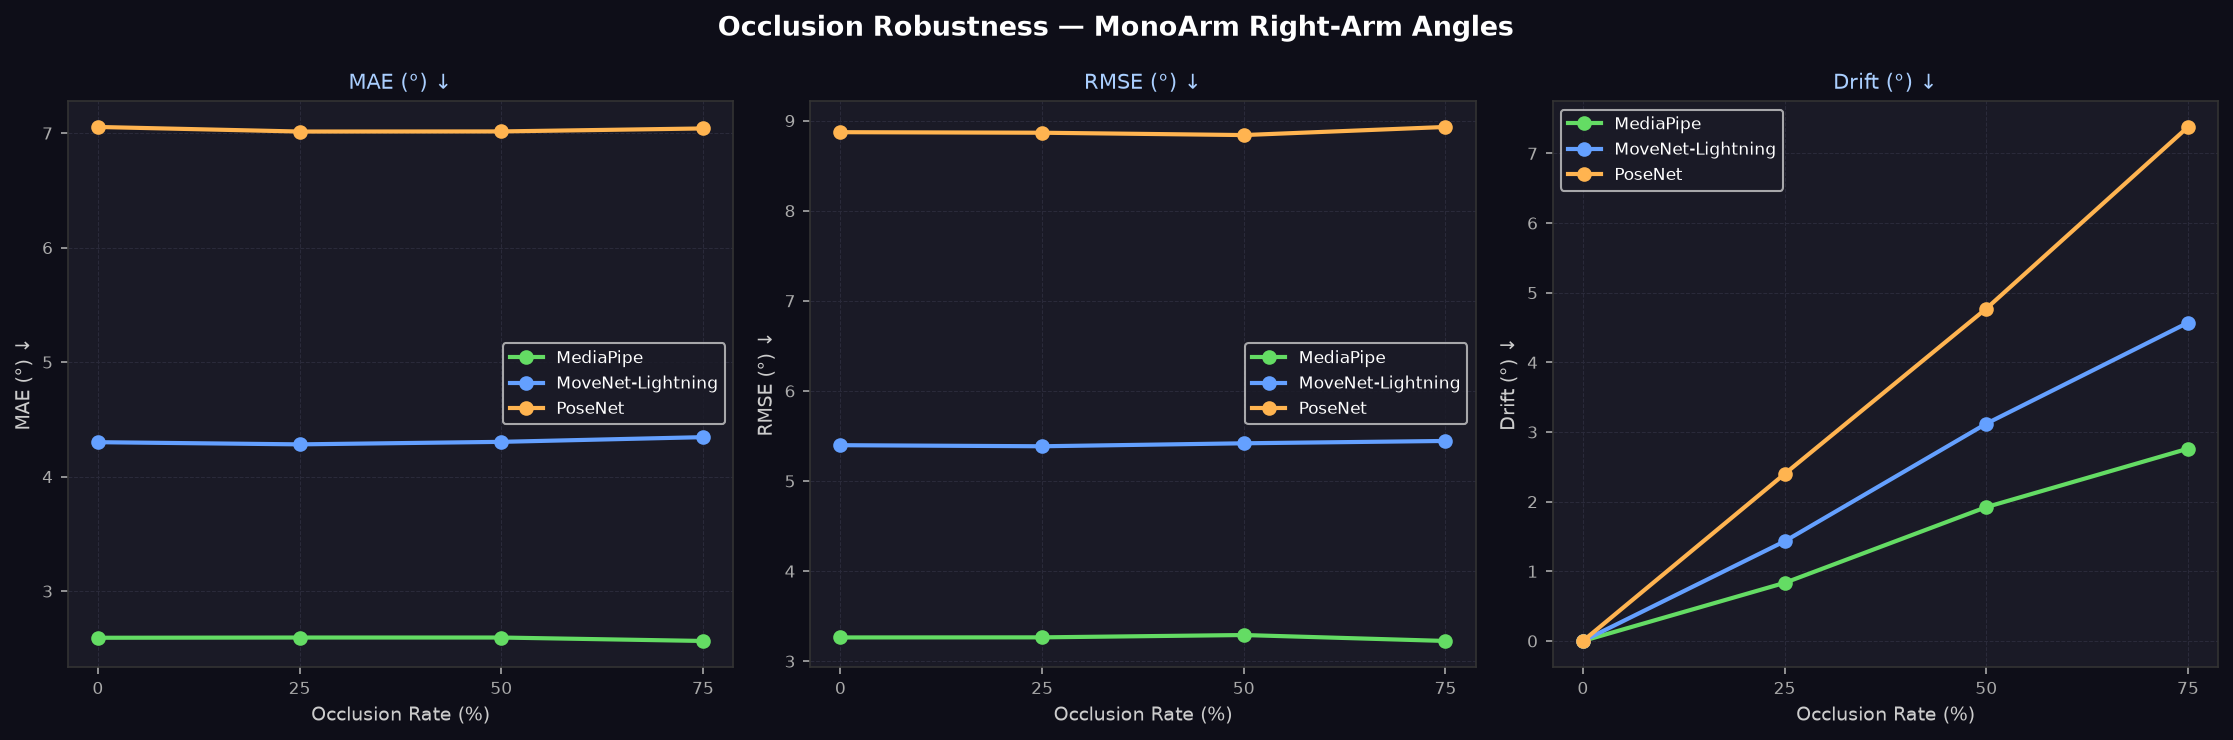
\includegraphics[width=\linewidth]{figures/occlusion_robustness.png}
\caption{Synthetic occlusion-robustness results
(Section~\ref{sec:results-occlusion}).}
\label{fig:occlusion}
\end{figure}

MAE and RMSE remain essentially flat as occlusion rises to 75\%, which is
a property of the metric rather than evidence of robustness: zero-order
hold repeats the last valid estimate, and against a slowly varying
trajectory a stale value is usually still close to the truth, so an
unconditional error average absorbs the loss. Drift -- the deviation
measured specifically over held frames -- grows close to linearly with
the occlusion rate for all three profiles, as expected of hold-based
dead reckoning against a moving target. We report both because the
contrast is the actionable result: a system evaluated only on aggregate
MAE would appear insensitive to tracking loss that drift exposes
immediately.

\subsection{End-to-End Verification on a Real Photograph}
\label{sec:results-real-frame}
The preceding experiments exercise the solver mathematics and pipeline
mechanics but not the neural estimator on real imagery. To close that
gap without dataset-scale access (Section~\ref{sec:dataset-access}), we
ran the real MediaPipe Pose Landmarker -- the same
\texttt{MediaPipeRunner} used throughout -- on one real photograph: frame
50 of the CMU Panoptic Studio sequence \texttt{171204\_pose1\_sample}
\cite{joo2015panoptic}, used strictly as an input image. Image decoding,
inference, torso-frame construction, bilateral decomposition, and the
Kalman update execute together, producing:

\begin{center}
\begin{tabular}{@{}lrrrr@{}}
\toprule
Side & Flex.\ (\textdegree) & Abd.\ (\textdegree) & Rot.\ (\textdegree) & Elbow (\textdegree) \\
\midrule
Right & $-35.25$ & $79.74$  & $151.58$ & $47.91$ \\
Left  & $-130.64$ & $71.76$ & $136.96$ & $34.02$ \\
\bottomrule
\end{tabular}
\end{center}

Rotation is flagged reliable on both sides (elbow flexion exceeds the
$25^\circ$ gate), and the filter update succeeds. The measured abduction
values ($79.7^\circ$ and $71.8^\circ$) are consistent with the pose
visible in Fig.~\ref{fig:realframe}, in which both arms are raised
laterally near shoulder height. This is a qualitative code-path
verification, not an accuracy measurement: no ground-truth angle for this
frame is used, and one frame cannot characterize an error distribution.

\begin{figure}[t]
\centering
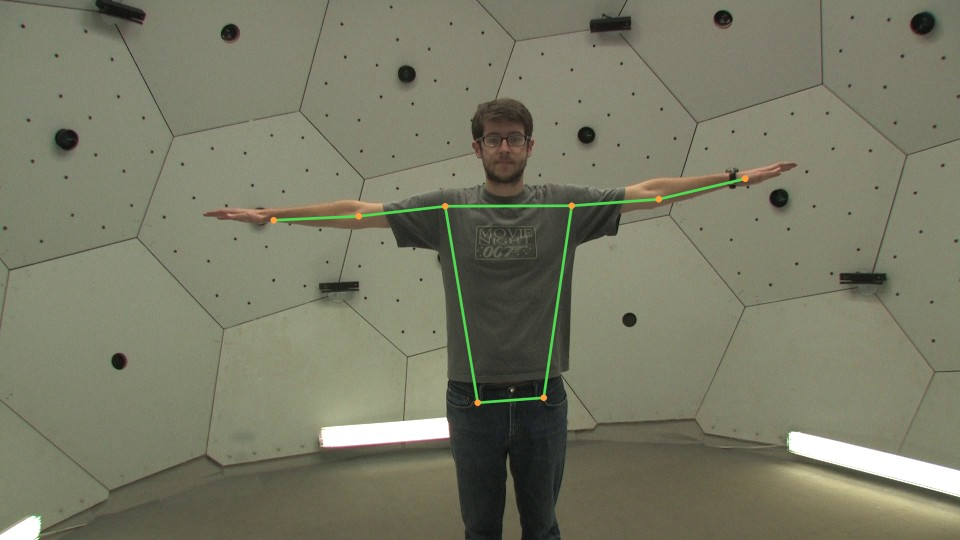
\includegraphics[width=\linewidth]{figures/real_frame_overlay.jpg}
\caption{Real MediaPipe landmarks (shoulders, elbows, wrists, hips)
overlaid on the input frame of Section~\ref{sec:results-real-frame}. The
subject is a Panoptic Studio capture participant included in that
dataset's public research release \cite{joo2015panoptic}, not a
participant recruited for this work.}
\label{fig:realframe}
\end{figure}

\subsection{Deployment Note: Runtime Dependencies}
The same verification surfaced two reproducibility hazards worth
recording. First, \texttt{mediapipe} 1.0.1 no longer ships the legacy
\texttt{mediapipe.solutions} API, so code written against it must fall
back to the Tasks API. Second, the Tasks API's native bindings load
\texttt{libEGL.so.1} and \texttt{libGLESv2.so.2} even for CPU-only
inference; on a headless container lacking those system libraries,
initialization fails with an error that names a graphics library rather
than the actual cause. Installing \texttt{libegl1} and \texttt{libgles2}
resolves it. Relatedly, the Tasks API requires strictly increasing frame
timestamps, which an integer-millisecond clock violates when consecutive
frames are processed within the same millisecond -- as happens in offline
loops over pre-extracted frames -- so the runner enforces monotonicity
explicitly.

\section{Discussion and Limitations}
\label{sec:limitations}

\subsection{Validation Scope}
\label{sec:dataset-access}
All results in Section~\ref{sec:results} are analytic checks on exactly
known geometry, synthetic-signal benchmarks with literature-calibrated
noise, or single-image code-path verification. None is a measurement of
MediaPipe, MoveNet, or PoseNet accuracy on real video against 3D ground
truth. That comparison requires Human3.6M \cite{ionescu2014human36m},
whose registration at \url{vision.imar.ro} we did not complete, or CMU
Panoptic Studio \cite{joo2015panoptic}, whose data server
(\texttt{domedb.perception.cs.cmu.edu}) was unreachable from our
development environment: both a plain GET and the HTTPS CONNECT tunnel
returned HTTP 403 under that environment's outbound network policy, while
other hosts remained reachable at the same time, indicating a
host-specific block rather than a connectivity failure. We report the
absence rather than substituting an unverified figure, because the
distinction between a measured and an assumed error is precisely what a
calibration reference must preserve.

The harness for that comparison is complete and shipped. With either
dataset available, results are produced by
\begin{verbatim}
python -m scripts.evaluate_h36m \
  --h36m_dir data/dataset/h3.6m/dataset \
  --frame_dir data/dataset/h3.6m/frames \
  --mode live \
  --frameworks mediapipe movenet_lightning posenet
\end{verbatim}
or, for the Panoptic substitute,
\begin{verbatim}
python -m scripts.evaluate_panoptic \
  --sequence_dir <extracted_panoptic_sequence> \
  --camera 00_00 \
  --frameworks mediapipe movenet_lightning posenet
\end{verbatim}
Both run the real estimators frame by frame, compute the metrics of
Section~\ref{sec:eval-harness}, execute the full statistical protocol,
and export a reproducibility record (library versions, git commit, random
seed, and the publication-grade flag) alongside the results. The Panoptic
path additionally runs a correlation-based temporal-alignment check
before scoring, since video and separately reconstructed motion-capture
streams paired by frame index are not guaranteed to share a common start.

\subsection{Geometric and Modeling Limits}
\textbf{Flexion near full abduction.} As $\theta_{abd}\to90^\circ$, both
$v_y$ and $v_z$ in $\theta_{flex}=\operatorname{atan2}(-v_z,-v_y)$
approach zero, making flexion acutely noise-sensitive. This is an
unavoidable coordinate pole of any two-angle parameterization of a
direction vector -- the rotational analogue of longitude at the
geographic poles -- and predicts degraded flexion accuracy specifically
near full abduction, independent of tracking quality.

\textbf{Rotation observability.} The forearm-proxy rotation estimate is
meaningful only above the elbow-flexion gate. Any monocular system using
a comparable proxy inherits this limit, and evaluations should report the
fraction of frames on which the estimate was geometrically valid rather
than an unconditional error.

\textbf{Depth ambiguity.} MediaPipe's pseudo-3D $z$ is a monocular
relative-depth estimate; MoveNet and PoseNet supply no depth at all.
Angle estimates from the latter two therefore rest more heavily on the 2D
projection and should be expected to be more view-dependent.

\textbf{Kinematic simplification.} The arm is modeled as two rigid
segments with a one-DOF elbow and a three-DOF shoulder, one of which is
proxied. This suffices for avatar control and reference signaling but
omits scapulohumeral rhythm and clavicular elevation, and is not a
biomechanically complete shoulder model.

\textbf{Exoskeleton integration.} The calibration module is structured
for reuse in exoskeleton sensor alignment, but no device was available to
validate that reuse; that remains future work.

\section{Conclusion}
We presented MonoArm, a monocular framework producing anatomically
consistent bilateral shoulder and elbow joint angles for real-time avatar
control, with full derivations of the torso frame, the ZXY decomposition
and its deliberate choice of singularity placement, the gated rotation
proxy, three causal filters, and a bounded-gain calibration. On a
synthetic benchmark the two-state Kalman filter achieved $0.55^\circ$
static deviation with no measurable step lag, and a 55-case analytic
suite verifies the solver, frame construction, filters, calibration
guards, and cross-framework keypoint remapping. Real-image inference
confirms the complete path executes end to end and yields angles
consistent with the observed pose. Accuracy against large-scale 3D
motion-capture ground truth remains unmeasured in this work because
neither reference dataset was reachable from our environment; the
evaluation harness, metric definitions, statistical protocol, and
alignment checks required for that comparison are delivered with the
system, making it a single documented command rather than a
reimplementation. Completing that validation, and then closing the loop
against a physical exoskeleton's joint encoders, are the natural next
steps.

\section*{Data and Code Availability}
All angle-solver, filter, calibration, streaming, and evaluation code,
the Unity project, and the 55-case test suite are part of this repository
(\texttt{python/}, \texttt{unity/}). Figures~\ref{fig:filters},
\ref{fig:occlusion}, and \ref{fig:realframe} are regenerated by
\texttt{python -m scripts.compare\_filters},
\texttt{python -m src.evaluation.occlusion\_test --synthetic}, and
\texttt{python -m scripts.verify\_real\_frame} respectively. No
license- or registration-gated dataset was used to produce any number
reported here. The single photograph in
Section~\ref{sec:results-real-frame}
(\texttt{docs/paper/figures/panoptic\_171204\_pose1\_sample\_frame50.jpg})
is frame 50 of CMU Panoptic Studio sequence
\texttt{171204\_pose1\_sample}, distributed by its maintainers as
``freely available for non-commercial and research purpose only''
conditional on citing a paper describing the dataset, satisfied here by
citing Joo~\textit{et al.}~\cite{joo2015panoptic}. The subject is a
participant in that public data-collection release, not a participant
recruited for this work, and the image serves solely as a code-path
verification input.

\begin{thebibliography}{00}

\bibitem{ionescu2014human36m}
C. Ionescu, D. Papava, V. Olaru, and C. Sminchisescu, ``Human3.6M: Large
scale datasets and predictive methods for 3D human sensing in natural
environments,'' \textit{IEEE Trans. Pattern Anal. Mach. Intell.}, vol.
36, no. 7, pp. 1325--1339, Jul. 2014.

\bibitem{joo2015panoptic}
H. Joo, H. Liu, L. Tan, L. Gui, B. Nabbe, I. Matthews, T. Kanade, S.
Nobuhara, and Y. Sheikh, ``Panoptic Studio: A massively multiview system
for social motion capture,'' in \textit{Proc. IEEE Int. Conf. Comput.
Vis. (ICCV)}, 2015, pp. 3334--3342.

\bibitem{bazarevsky2020blazepose}
V. Bazarevsky, I. Grishchenko, K. Raveendran, T. Zhu, F. Zhang, and M.
Grundmann, ``BlazePose: On-device real-time body pose tracking,''
\textit{arXiv preprint arXiv:2006.10204}, 2020.

\bibitem{movenet2021blog}
R. Votel and N. Li, ``Next-generation pose detection with MoveNet and
TensorFlow.js,'' \textit{TensorFlow Blog}, May 2021. [Online]. Available:
\url{https://blog.tensorflow.org/2021/05/next-generation-pose-detection-with-movenet-and-tensorflowjs.html}

\bibitem{papandreou2018personlab}
G. Papandreou, T. Zhu, L.-C. Chen, S. Gidaris, J. Tompson, and K. Murphy,
``PersonLab: Person pose estimation and instance segmentation with a
bottom-up, part-based, geometric embedding model,'' in \textit{Proc. Eur.
Conf. Comput. Vis. (ECCV)}, 2018, pp. 269--286.

\bibitem{wu2005isb}
G. Wu \textit{et al.}, ``ISB recommendation on definitions of joint
coordinate systems of various joints for the reporting of human joint
motion---Part II: shoulder, elbow, wrist and hand,'' \textit{J. Biomech.},
vol. 38, no. 5, pp. 981--992, 2005.

\bibitem{biryukova2000kinematics}
E. V. Biryukova, A. Roby-Brami, A. A. Frolov, and M. Mokhtari,
``Kinematics of human arm reconstructed from spatial tracking system
recordings,'' \textit{J. Biomech.}, vol. 33, no. 8, pp. 985--995, 2000.

\bibitem{koritnik2003kinematic}
T. Koritnik, T. Bajd, and M. Munih, ``A simple kinematic model of a human
body for virtual environments,'' Faculty of Electrical Engineering,
University of Ljubljana. [Online]. Available:
\url{https://www.researchgate.net/publication/226438496}

\bibitem{kalman1960new}
R. E. Kalman, ``A new approach to linear filtering and prediction
problems,'' \textit{J. Basic Eng.}, vol. 82, no. 1, pp. 35--45, 1960.

\bibitem{savitzky1964smoothing}
A. Savitzky and M. J. E. Golay, ``Smoothing and differentiation of data
by simplified least squares procedures,'' \textit{Anal. Chem.}, vol. 36,
no. 8, pp. 1627--1639, 1964.

\bibitem{yang2011articulated}
Y. Yang and D. Ramanan, ``Articulated pose estimation with flexible
mixtures-of-parts,'' in \textit{Proc. IEEE Conf. Comput. Vis. Pattern
Recognit. (CVPR)}, 2011, pp. 1385--1392.

\bibitem{mehta2017vnect}
D. Mehta \textit{et al.}, ``VNect: Real-time 3D human pose estimation
with a single RGB camera,'' \textit{ACM Trans. Graph.}, vol. 36, no. 4,
Jul. 2017.

\bibitem{bland1986statistical}
J. M. Bland and D. G. Altman, ``Statistical methods for assessing
agreement between two methods of clinical measurement,'' \textit{Lancet},
vol. 327, no. 8476, pp. 307--310, 1986.

\bibitem{wilcoxon1945individual}
F. Wilcoxon, ``Individual comparisons by ranking methods,''
\textit{Biometrics Bull.}, vol. 1, no. 6, pp. 80--83, 1945.

\bibitem{holm1979simple}
S. Holm, ``A simple sequentially rejective multiple test procedure,''
\textit{Scand. J. Stat.}, vol. 6, no. 2, pp. 65--70, 1979.

\bibitem{cohen1988statistical}
J. Cohen, \textit{Statistical Power Analysis for the Behavioral
Sciences}, 2nd ed. Hillsdale, NJ, USA: Lawrence Erlbaum Associates, 1988.

\end{thebibliography}

\end{document}
